\documentclass[10pt,aspectratio=149]{beamer}
\usecolortheme{Calm}
\usetheme{Calm}
%\usefonttheme[onlymath]{serif} % beamer force les maths en cmss par défaut, qui n'a pas de vrai gras : \mathbf{} restait fin
\usepackage{amsmath}
\usepackage{pgfplots}
\pgfplotsset{compat=1.18}
\usepackage{pgfplotstable}
\usepackage[utf8]{inputenc}
\usepackage{hyperref}
\RequirePackage[absolute,overlay]{textpos}
%\usepackage[sfdefault]{cabin}
%\usepackage[T1]{fontenc}
%\setlength{\TPHo{}rizModule}{\paperwidth}
%\setlength{\TPVertModule}{\paperheight}
%\definecolor{OQEdarkblue}{HTML}{046085}


\defbeamertemplate*{background canvas}{bg}
{%
  \color{lightgray!40}\vrule width\paperwidth height\paperheight% added bg color
}

% Centered, larger display equation
\newcommand{\keyeq}[1]{%
  \begin{center}
    \Large$\displaystyle #1$
  \end{center}%
}

% Same style, for a system of equations aligned on "="
% (rows separated by \\, each row written as LHS &= RHS)
\newcommand{\keyeqs}[1]{%
  \begin{center}
    \normalsize$\displaystyle
    \begin{aligned}
    #1
    \end{aligned}
    $
  \end{center}%
}

%------------------------------

\author{Dominique Gravel}
\title{Metacommunities, distribution and competition}
\date{August 26th, 2026}
\institute{Université de Sherbrooke \\ Summer school in biodiversity modelling}

%------------------------------
% TITLE SLIDE
%------------------------------

\usebackgroundtemplate
{
  
\includegraphics[width=\paperwidth,height=\paperheight]{bg}%
}

\begin{document}

	\begin{frame}[plain]
		\titlepage
	\end{frame}

%------------------------------
% INTRO
%------------------------------

%------------------------------

\begin{frame}

    \begin{center}
        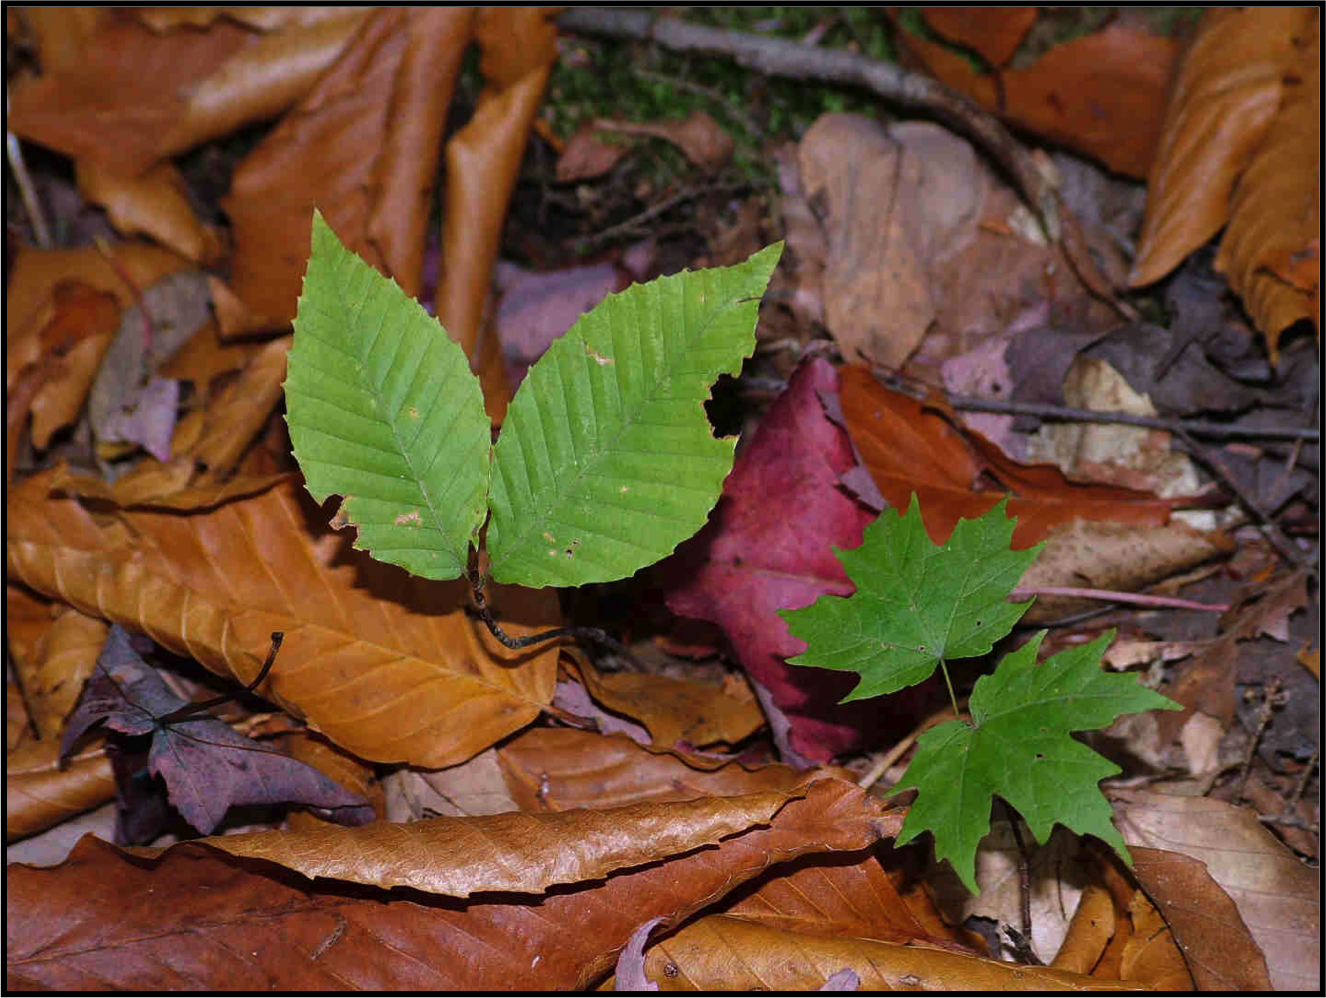
\includegraphics[height=0.7\textheight]{Figs/seedlings}\\
    \end{center}

\end{frame}

%------------------------------

\begin{frame}{Recall}

    \begin{center}
        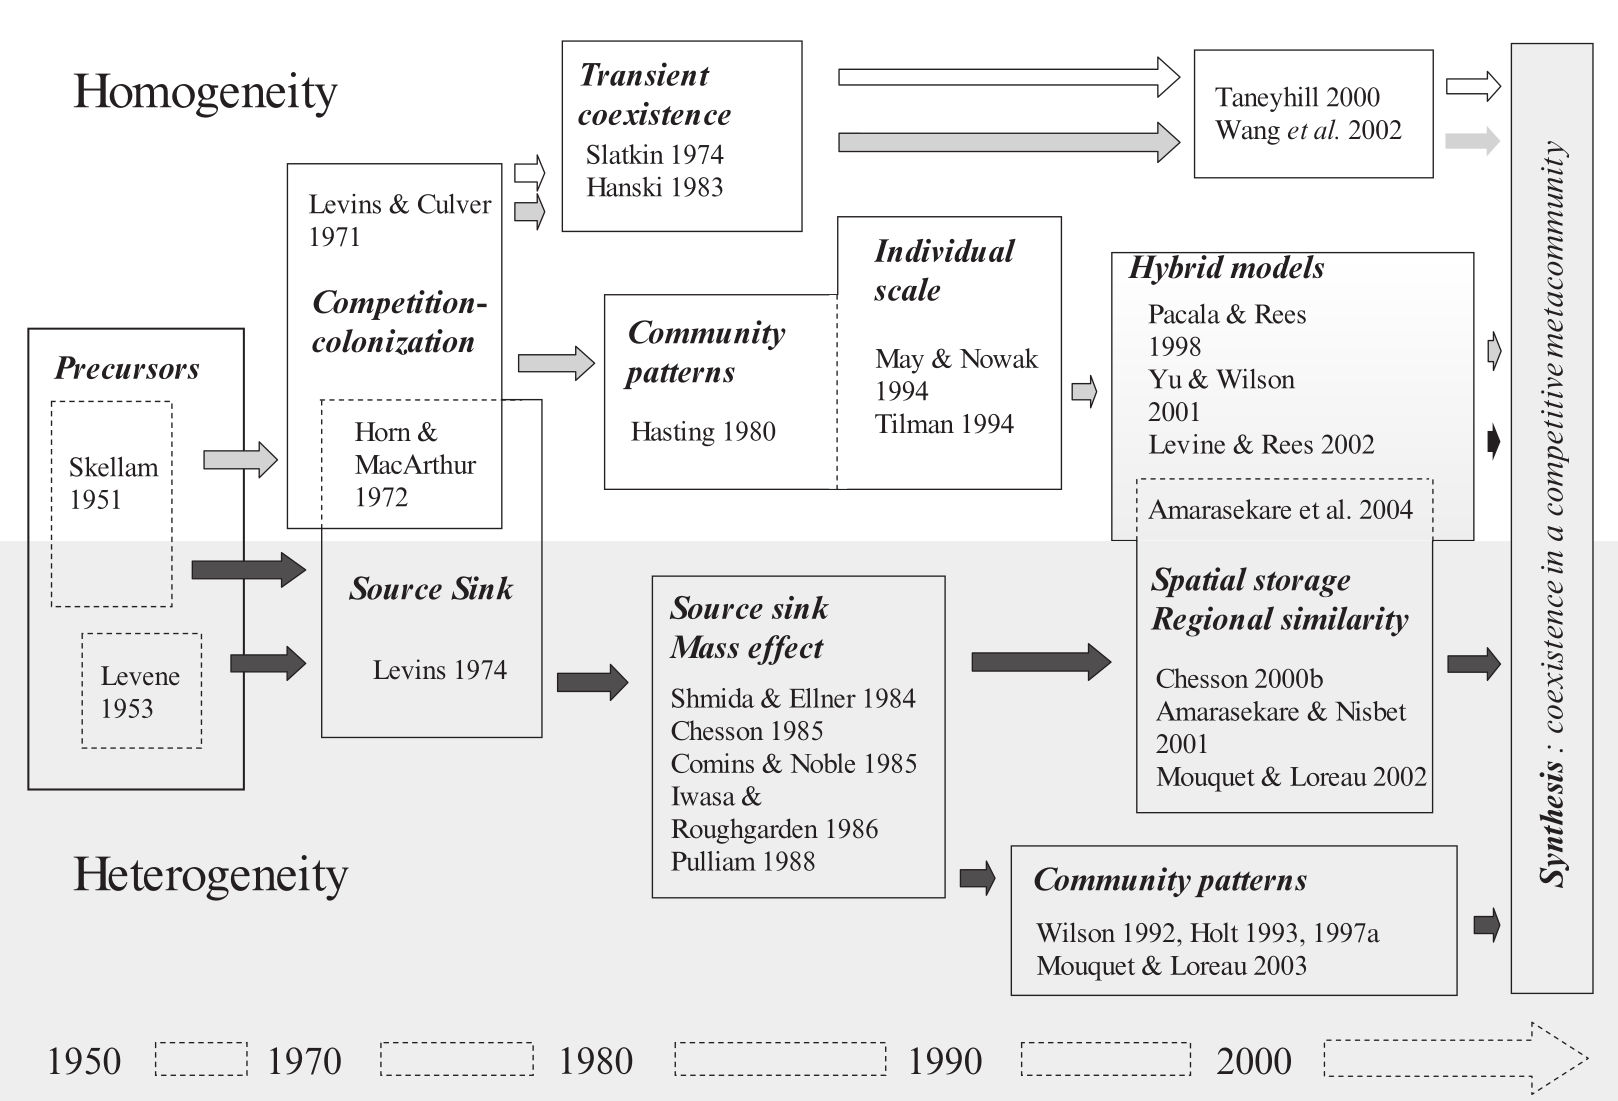
\includegraphics[height=0.7\textheight]{Figs/mouquet2005}\\
        \footnotesize Mouquet et al. 2005 in Holyoak et al. Metacommunity Ecology. Chicago University Press
    \end{center}

\end{frame}

%------------------------------

\begin{frame}[fragile]{Definition}

    \LARGE \textit{A set of local communities that are linked by dispersal of multiple potentially interacting species}\\
    \footnotesize Leibold et al. 2004. Eco. Lett 

\end{frame}

%------------------------------

\begin{frame}{Definition}

    \begin{center}
        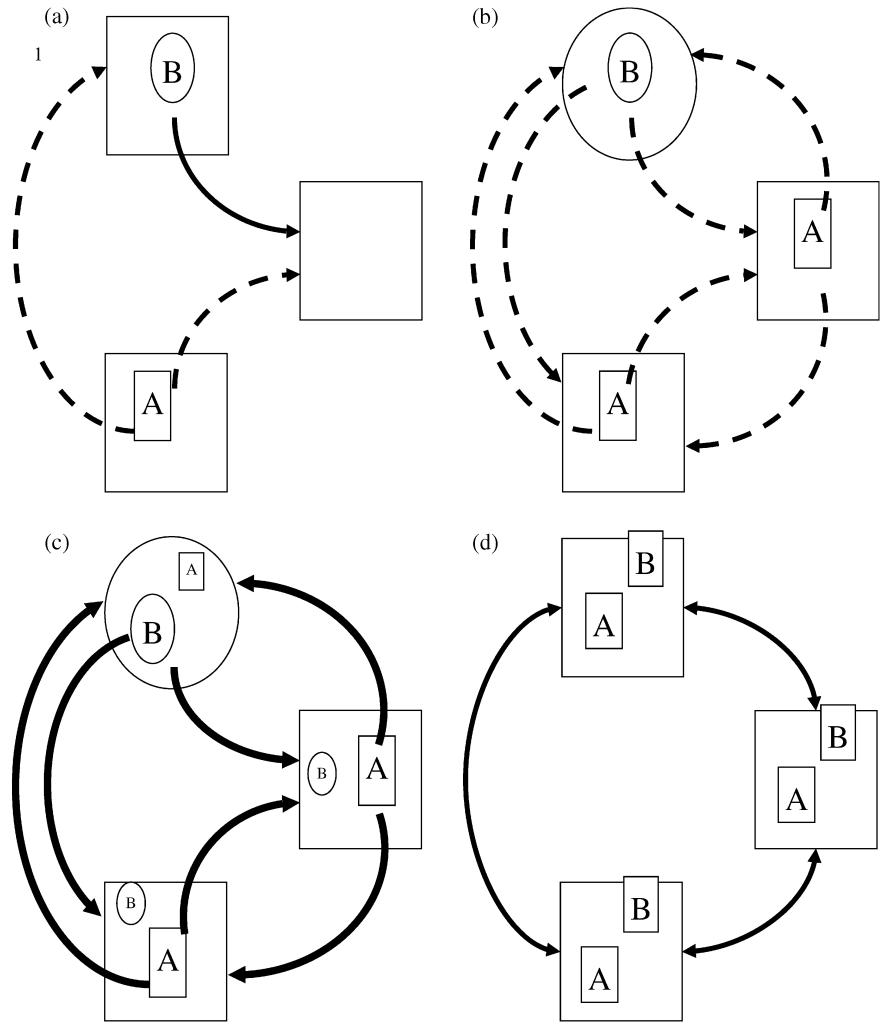
\includegraphics[height=0.7\textheight]{Figs/leibold2004}\\
        \footnotesize Leibold et al. 2004. Eco. Lett 
    \end{center}

\end{frame}

%------------------------------

\begin{frame}{Patch dynamics}

	\begin{columns}
		\begin{column}{0.5\textwidth}
            \textit{A perspective that assumes that patches are identical and that each patch is capable of containing
            populations. Patches may be occupied or unoccupied. Local species diversity is limited by dispersal.
            Spatial dynamics are dominated by local extinction and colonization}
		\end{column}
%----
		\begin{column}{0.5\textwidth}
            \begin{center}
                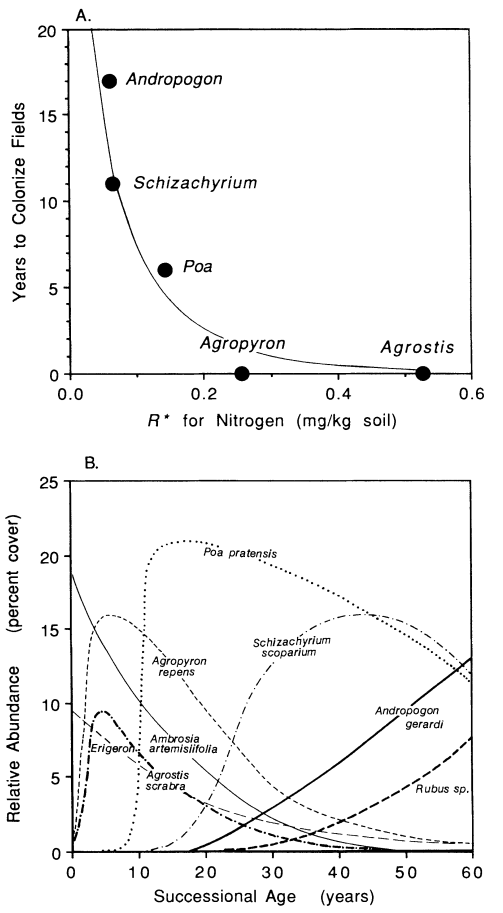
\includegraphics[height=0.7\textheight]{Figs/tilman1994} 
            \end{center}
		\end{column}
	\end{columns}

\end{frame}

%------------------------------

\begin{frame}{Neutral theory}

	\begin{columns}
		\begin{column}{0.5\textwidth}
            \textit{A perspective in which all species are similar in their competitive ability, movement and fitness
            (Hubbell 2001). Population interactions among species consist of random walks that alter relative
            frequencies of species. The dynamics of species diversity are then derived both from probabilities of
            species loss (extinction, emigration) and gain (immigration, speciation).}
		\end{column}
%----
		\begin{column}{0.5\textwidth}
            \begin{center}
                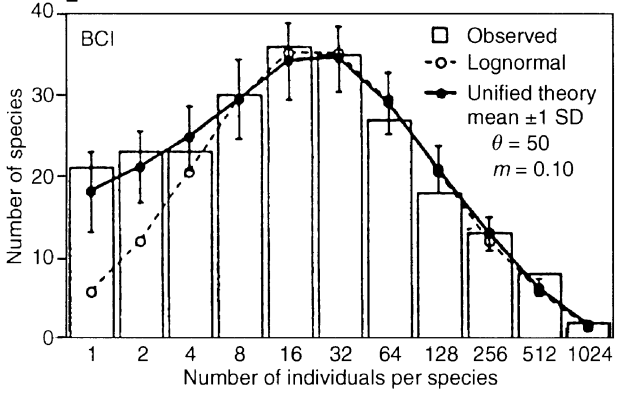
\includegraphics[height=0.5\textheight]{Figs/hubbell1997} 
            \end{center}
		\end{column}
	\end{columns}

\end{frame}

%------------------------------

\begin{frame}{Species sorting}

	\begin{columns}
		\begin{column}{0.5\textwidth}
            \textit{A perspective that emphasizes the resource gradients or patch types cause sufficiently strong
            differences in the local demography of species and the outcomes of local speciesÕ interactions that
            patch quality and dispersal jointly affect local community composition. This perspective emphasizes
            spatial niche separation above and beyond spatial dynamics. Dispersal is important because it allows
            compositional changes to track changes in local environmental conditions}
		\end{column}
%----
		\begin{column}{0.5\textwidth}
            \begin{center}
                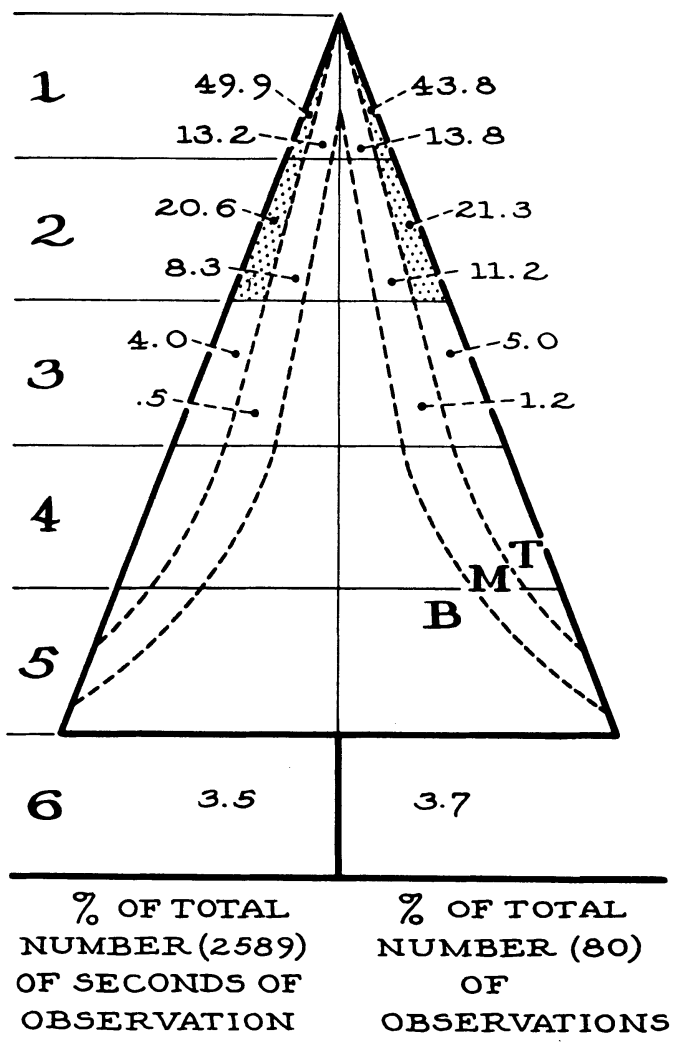
\includegraphics[height=0.7\textheight]{Figs/macarthur1958} 
            \end{center}
		\end{column}
	\end{columns}

\end{frame}

%------------------------------

\begin{frame}{Mass effect}

	\begin{columns}
		\begin{column}{0.5\textwidth}
            \textit{A perspective that focuses on the effect of immigration and emigration on local population dynamics.
            In such a system species can be rescued from local competitive exclusion in communities where they
            are bad competitors, by immigrate from communities where they are good competitors. This
            perspective emphasizes the role that spatial dynamics affect local population densities.}
		\end{column}
%----
		\begin{column}{0.5\textwidth}
            \begin{center}
                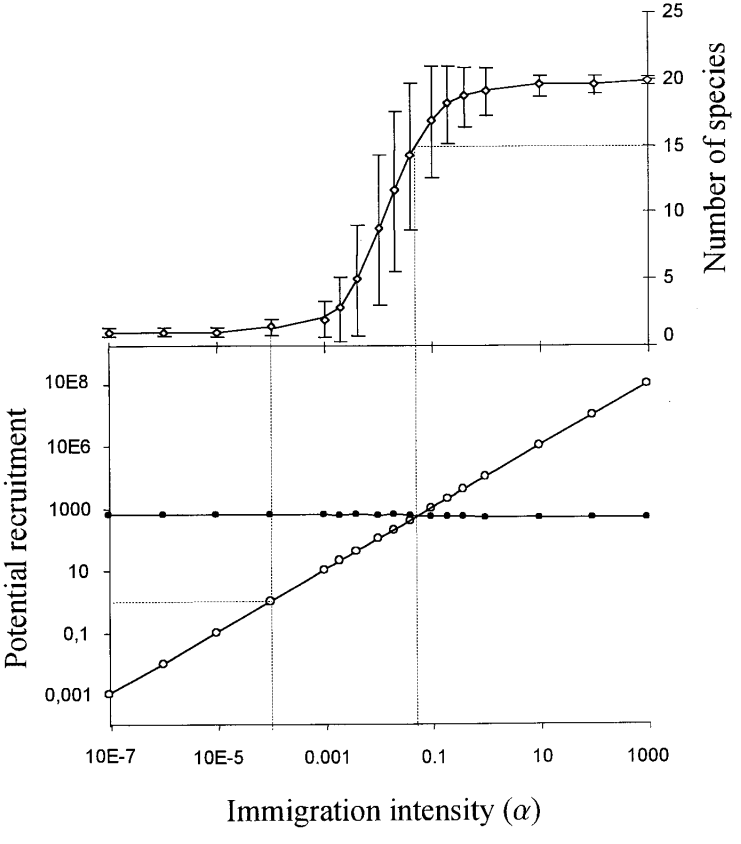
\includegraphics[height=0.7\textheight]{Figs/loreau1999} 
            \end{center}
		\end{column}
	\end{columns}

\end{frame}

%------------------------------

{
\usebackgroundtemplate{}
\begin{frame}

	\pagecolor{BDQC1st}
	\color{white}

	\LARGE{\textit{Discussion}}

\end{frame}
}

%------------------------------

\begin{frame}{Neutral model}{Verbal description}

    \begin{itemize}
        \item Consider a lattice with each cell occupied by a single individual
        \item Time scale corresponds to the replacement of 1 individual at a time
        \item All species have the same probability of mortality
        \item Compute number of seeds reaching a seed trap at the center of the cell
        \item Dispersal occurs from neighbours with probability (1-m) and from a regional pool with probability m
        \item For simplicity, all species have the same abundance in the regional pool
        \item All species produce the same number of seeds
        \item Recruitment occurs by selecting a seed at random from the seed trap
        \item Repeat for a (very) large number of time steps
    \end{itemize}

\end{frame}

%------------------------------

\begin{frame}[fragile]{Neutral model}{Pseudo-code}

    \begin{verbatim}
        SET run parameters $l$, $s$, $nsteps$
        SET ecological parameters $m$ and $r$
    
        DEFINE array XY of spatial coordinates of size $l^2$ 
        DEFINE array J of size $l^2 x S$
    
        COMPUTE connectivity matrix ConMat 
    
        FOR n in 1:nsteps
            SELECT a cell z at random 
                J[z] = 0
            COMPUTE replacement probability for each species
            DRAW a species identity using multinomial distribution
            UPDATE array J
    \end{verbatim}

\end{frame}

%------------------------------

\begin{frame}[fragile]{Neutral model}{Replacement probability}

    \begin{verbatim}
        # Local replacement 
            n_propagules = ContMat%*%J
            p_local = n_propagules/(r^2-1)

        # Regional replacement 
            p_regional = 1/s

        # Final probability
            p = (1-m)*p_local + m*p_regional
    \end{verbatim}

\end{frame}

%------------------------------

{
\usebackgroundtemplate{}
\begin{frame}

	\pagecolor{BDQC1st}
	\color{white}

	\LARGE{\textit{Add species differences}}

\end{frame}
}

%------------------------------

\begin{frame}{Species sorting}{Verbal description}

    \begin{itemize}
        \item Consider that each cell has a unique environmental condition between 0 and 1
        \item The local environment impacts seed germination 
        \item Response to the environment is unimodal
        \item Each speices has a niche optimum between 0 and 1
        \item All species have the same niche width
    \end{itemize}

\end{frame}

%------------------------------

\begin{frame}[fragile]{Species sorting}{Additions to code}

    \begin{verbatim}
        # Local replacement 
            n_propagules = ContMat%*%J
            survival = survival_fn(E,O,sigma)
            p_local = survival * n_propagules/(r^2-1)
    \end{verbatim}

\end{frame}

%------------------------------

{
\usebackgroundtemplate{}
\begin{frame}

	\pagecolor{BDQC1st}
	\color{white}

	\LARGE{\textit{Compare expectations}}

\end{frame}
}

%------------------------------

\begin{frame}{Simulations}

    \begin{itemize}
        \item Local abundance distribution at equilibrium 
        \item Regional abundance distribution at equilibrium
        \item Species area relationship
        \item Shared species as a function of distance 
        \item Species-environment relationship
    \end{itemize}

\end{frame}

%------------------------------

\begin{frame}{Advanced}

    \begin{itemize}
        \item Compare different spatial autocorrelations to evaluate the effect of mass effect
        \item Think about a way to incorporate competition-colonization trade-off
    \end{itemize}

\end{frame}

%------------------------------

\begin{frame}{Advanced}{Other topics}

    \begin{itemize}
        \item Null hypothesis or a baseline ?
        \item Discriminating paradigms
        \item Quasi-neutral models
        \item Continuous vs discrete organization
        \item Spatial network of patches
        \item Spatial contingency
        \item Disturbances
        \item Speciation model (point mutation, random fission, protracted, reproductive isolation)
        \item Phylogeny
        \item From genes to communities
        \item Moments of metacommunities
    \end{itemize}

\end{frame}

%------------------------------
%------------------------------
%------------------------------
\end{document}
